% =========================================================================
% Secao 3 - Dados e metodo
% =========================================================================

\section{Dados e método}
\label{sec:dados_metodo}

A Pesquisa Nacional por Amostra de Domicílios Contínua (PNADC),
conduzida trimestralmente pelo IBGE desde o primeiro trimestre de
2012, baseia-se em uma amostra probabilística de cerca de 211 mil
domicílios e cobre, em cada trimestre, aproximadamente 460 mil
pessoas residentes no Brasil. A pesquisa substituiu a PNAD anual e
adotou um \emph{design} de painel rotativo, em que cada domicílio
selecionado é entrevistado em cinco trimestres consecutivos. O
esquema amostral é tecnicamente descrito como 1-2(5), conforme
detalhamos a seguir, e essa estrutura determina tanto o que é
possível observar no painel longitudinal quanto o que pode ser
distorcido pelo calendário escolar.

\subsection{O esquema rotativo da PNADC}
\label{ssec:rotativo}

A PNADC adota um esquema rotativo do tipo 1-2(5), no qual cada
domicílio selecionado permanece na amostra por cinco trimestres
consecutivos, com uma entrevista por trimestre. Os domicílios entram
e saem em fluxo contínuo, organizados em grupos de rotação indexados
pela variável \texttt{V1014}. Em cada trimestre, um quinto dos
domicílios entra na amostra, ocupando a primeira visita, enquanto
outro quinto sai, após completar a quinta visita. As cinco visitas
a um mesmo domicílio são separadas por intervalos de aproximadamente
três meses, o que resulta em um horizonte máximo de acompanhamento
individual de cerca de quinze meses.

A Figura~\ref{fig:esquema_rotativo} ilustra a estrutura do esquema.
Cada linha corresponde a uma rotação e cada célula a uma das cinco
visitas (V1 a V5) ao mesmo domicílio. A trajetória depende
exclusivamente do trimestre de entrada. Um domicílio que entra no
primeiro trimestre do ano $y$ (rotação 1) é entrevistado em $Q_1$,
$Q_2$, $Q_3$ e $Q_4$ desse mesmo ano e, finalmente, no $Q_1$ do
ano $y+1$, totalizando cinco visitas. Um domicílio que entra em
$Q_2$ (rotação 2) é entrevistado em $Q_2$, $Q_3$ e $Q_4$ de $y$ e
em $Q_1$ e $Q_2$ de $y+1$. De forma análoga, rotação 3 é
entrevistada em $Q_3$ e $Q_4$ de $y$ e em $Q_1$, $Q_2$ e $Q_3$ de
$y+1$, e rotação 4 aparece em $Q_4$ de $y$ e em $Q_1$, $Q_2$,
$Q_3$ e $Q_4$ de $y+1$.

\begin{figure}[htbp]
\centering
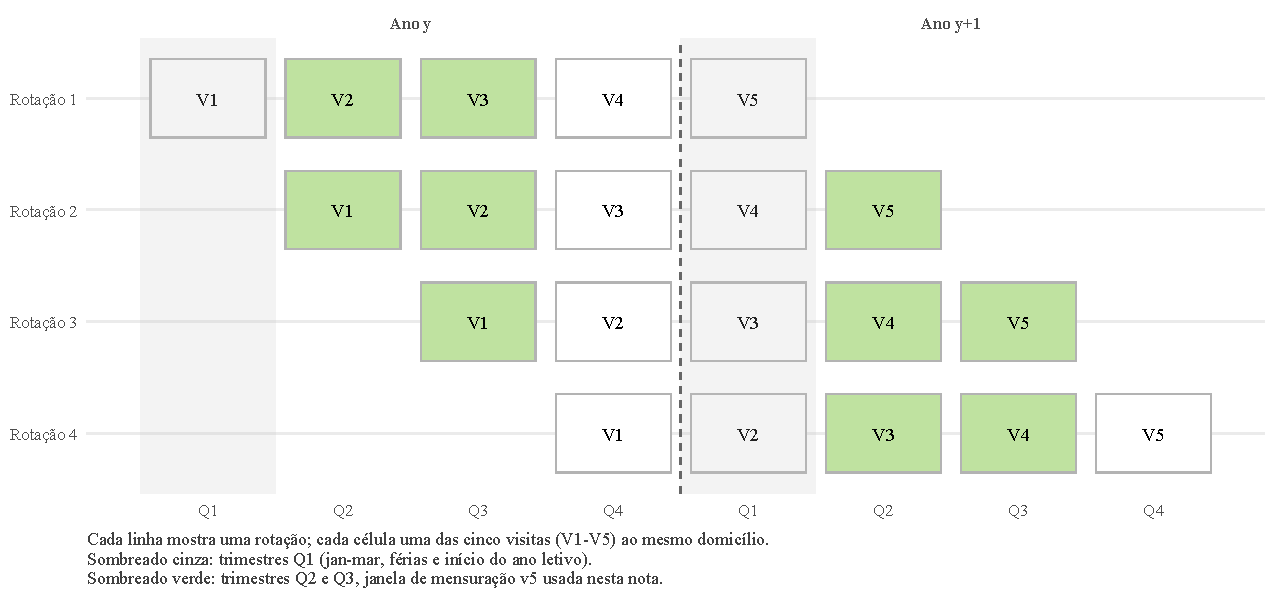
\includegraphics[width=0.95\textwidth]{../DataWork/5_Figures/output/F0_esquema_rotativo.pdf}
\caption{Esquema rotativo 1-2(5) da PNADC e janela de mensuração v5.}
\label{fig:esquema_rotativo}
\figurenote{Cada linha é uma rotação; cada célula é uma das cinco
visitas (V1--V5) ao mesmo domicílio. A faixa cinza marca os
trimestres $Q_1$ (jan-mar), período de férias e início do ano
letivo. A faixa verde marca $Q_2$ e $Q_3$, janela de mensuração v5
adotada nesta nota. Rotação 1 (entra em $Q_1$ do ano $y$) só tem
observação em $Q_1$ de $y+1$, ficando portanto excluída por
construção da medição entre-anos v5.}
\end{figure}

A consequência imediata desse esquema é que, para qualquer
domicílio do painel, sempre existe pelo menos uma observação em
dois anos calendário consecutivos. Em outras palavras, todo
domicílio necessariamente atravessa a virada de ano, o que torna a
PNADC um instrumento naturalmente vocacionado para medir transições
entre anos letivos. Há, contudo, uma assimetria importante.
Independentemente do trimestre de entrada, a primeira observação
no ano $y+1$ ocorre quase sempre no $Q_1$ desse ano. Em termos
práticos, isso significa que, sem ajuste metodológico, mais de
noventa por cento das transições $t \to t+1$ seriam medidas com
observação em $t+1$ em janeiro, fevereiro ou março, exatamente o
período em que o ano letivo brasileiro está em férias ou em sua
fase inicial. Para evitar esse viés, esta nota restringe a janela
de medição entre-anos aos trimestres $Q_2$ e $Q_3$ de cada ano,
indicados em verde na Figura~\ref{fig:esquema_rotativo}.
Domicílios de rotação 1, que não têm nenhuma observação em $Q_2$
ou $Q_3$ do ano $y+1$, são por construção excluídos da medição
entre-anos. A discussão completa do efeito-férias e das alternativas
metodológicas está na Seção~\ref{ssec:efeito_ferias}.

Esse \emph{design} cria duas janelas naturais para medir o fluxo
escolar. A janela intra-ano corresponde à primeira e à última
observação de um mesmo indivíduo dentro de um ano calendário,
separadas tipicamente por dois a quatro trimestres, e captura
saídas da escola que ocorreram dentro do ano letivo, o conceito
operacional de abandono. A janela entre-anos corresponde a uma
observação em $Q_2$ ou $Q_3$ de um ano calendário e a observação
correspondente em $Q_2$ ou $Q_3$ do ano seguinte, e captura
transições entre anos letivos, abrangendo os conceitos de evasão,
promoção, repetência e migração para EJA.

A construção do painel exige duas operações, a saber, a
identificação estável do domicílio entre visitas e a identificação
estável de cada pessoa dentro do domicílio. Construímos o
identificador de domicílio como a concatenação de quatro variáveis,
isto é, unidade federativa (\texttt{UF}), unidade primária de
amostragem (\texttt{UPA}), número de seleção do domicílio dentro
da UPA (\texttt{V1008}) e número do painel (\texttt{V1014}).
Domicílios pertencentes ao mesmo painel são entrevistados nos
mesmos cinco trimestres consecutivos, de modo que a chave
\texttt{UF + UPA + V1008 + V1014} é estável por construção e
identifica o domicílio através das visitas. Dentro de cada
domicílio, a posição da pessoa na lista de moradores é codificada
pela variável \texttt{V2003}. O \emph{matching} preliminar de uma
mesma pessoa entre visitas usa, portanto, a combinação
\texttt{hh\_id + V2003}. Como \texttt{V2003} pode variar caso haja
entrada ou saída de moradores entre visitas, implementamos três
camadas de validação por sexo (\texttt{V2007}), idade (\texttt{V2009})
e reconciliação por correspondência de atributos. Indivíduos com elo
válido em pelo menos duas visitas formam o painel, e as taxas de
\emph{matching} obtidas estão reportadas na
Seção~\ref{ssec:atrito}. Os detalhes operacionais das três camadas
de validação estão no Apêndice~\ref{app:variaveis}.

Os pesos amostrais da PNADC trimestral, codificados na variável
\texttt{V1028}, são calibrados para representatividade trimestral,
e não longitudinal. Para indicadores de fluxo, usamos o peso da
primeira observação do indivíduo no painel, esquema que designamos
por P1. Reportamos um teste de robustez na
Seção~\ref{ssec:atrito} usando reponderação por \emph{inverse
propensity} para corrigir atrito, seguindo a metodologia padrão
de painel rotativo.\footnote{A literatura sobre reponderação em
painéis com atrito foi formalizada por
\citet{wooldridge_2007_attrition} e adaptada para a PNADC em
\citet{IPEA2022_painel}.} Para evitar células com imprecisão
excessiva, suprimimos das tabelas qualquer combinação (subgrupo,
indicador, ano) com $N < 30$. Reportamos $N$ efetivo em todas as
tabelas e o intervalo de confiança \emph{bootstrap}, com
\emph{cluster} em UPA, nas tabelas principais.

\begin{caixatexto}{Caixa 1: Uma família ao longo dos cinco trimestres}
Para fixar ideias, considere a família M., entrevistada pela PNADC
pela primeira vez em 2023Q2 (rotação 2). O domicílio é identificado
pela combinação \texttt{UF=33, UPA=001234567, V1008=05, V1014=02}.
Na primeira visita, o domicílio tem cinco moradores, a saber, o
casal M., com 40 e 38 anos respectivamente, e três filhos, isto é,
Pedro, de 16 anos, no primeiro ano do EM; Maria, de 13 anos, no
oitavo ano do EF; e João, de 7 anos, no segundo ano do EF. Em
2023Q2, Pedro estuda (\texttt{V3002=1}) em escola estadual
(\texttt{V3002A=3}) no primeiro ano do EM (\texttt{V3006=1}). Em
2023Q3, Pedro mantém a mesma série, confirmando a observação. Em
2024Q2 (quinta visita), Pedro tem 17 anos e responde
\texttt{V3002=1} (frequenta) no segundo ano do EM
(\texttt{V3006=2}), tendo sido promovido entre 2023 e 2024.

A linkagem produz duas observações no painel longitudinal. A
primeira é o registro de Pedro em $Q_2$ ou $Q_3$ de 2023 com
nível 10 (1º ano do EM). A segunda é o registro de Pedro em
$Q_2$ de 2024 com nível 11 (2º ano do EM). Como nível em $t+1$ é
superior a nível em $t$, a transição é classificada como
promoção. Se Pedro estivesse, ao invés disso, sem matrícula em
2024Q2 mas com $V3014=1$ (concluiu o curso anterior), seria
classificado como promoção mesmo sem matrícula posterior, em
alinhamento com a definição do INEP para conclusão do EM. E se
ele estivesse frequentando uma escola privada em 2024, apareceria
com $V3002A=1$, ainda contado como promoção, mas com a mudança de
rede pública para privada visível apenas para a PNADC, não para
o Censo Escolar. Essa é a essência da captura de retorno.
\end{caixatexto}

\subsection{Harmonização de variáveis educacionais}

A PNADC mudou o nome e o significado dos códigos de algumas
variáveis educacionais em 2016. Especificamente, na variável
\texttt{V3003} pré-2016, o código 3 representava ``Regular
Fundamental'', o código 5 ``Regular Médio'' e o código 7
``Educação Profissional Médio'', enquanto na variável
\texttt{V3003A} pós-2016, os mesmos conceitos são representados
pelos códigos 4, 6 e 7, respectivamente. Esta nota harmoniza as
duas codificações em \texttt{etapa\_consolid}, conforme detalhado
no Apêndice~\ref{app:variaveis}. A Tabela~\ref{tab:harmonizacao}
resume o mapeamento das principais variáveis entre as duas versões.

\begin{table}[htbp]
\centering
\caption{Harmonização de variáveis educacionais entre versões da PNADC}
\label{tab:harmonizacao}
\begin{tabular}{lll}
\toprule
Conceito                                 & Versão pré-2016 & Versão 2016+    \\
\midrule
Frequenta escola                         & V3002           & V3002           \\
Rede da escola                           & V3002A          & V3002A          \\
Curso/etapa que frequenta                & V3003 (códigos 3, 5, 7) & V3003A (códigos 4, 6, 7) \\
Série/ano que frequenta                  & V3006 & V3006 \\
Concluiu o curso? (último frequentado)   & V3014 & V3014 \\
Último ano/série concluído               & V3013 & V3013A \\
\bottomrule
\end{tabular}
\end{table}

Na harmonização, \texttt{etapa\_consolid} consolida o curso em
códigos uniformes para todo o período. Da \texttt{etapa\_consolid}
e da \texttt{V3006}, derivamos a variável de \emph{nível}, um
índice ordinal monotônico que combina etapa e série. Valores de
um a cinco correspondem aos anos do EF iniciais, seis a nove aos
anos do EF finais, dez a doze aos três anos do EM regular, e
treze ao quarto ano do EM técnico, que existe em parte dos cursos
de educação profissional integrada. A macroetapa, derivada do
nível, distingue EF iniciais (níveis 1 a 5), EF finais (níveis 6
a 9) e Ensino Médio (níveis 10 a 13, regular ou técnico). EJA EF
e EJA EM são tratadas como modalidades separadas, fora do painel
principal mas reportadas em apêndice.

\subsection{Definições operacionais dos cinco indicadores}
\label{ssec:definicoes}

Os cinco indicadores são, em palavras, os seguintes. O abandono é
a fração de alunos matriculados em regular EF ou EM regular ou
técnico na primeira observação do ano $t$ que apresenta
$\text{freq}=0$ na última observação do mesmo ano $t$. Mudança
de modalidade dentro do ano, especificamente do EM regular para
EJA, é tratada como migração para EJA intra-ano, não como
abandono. A migração para EJA entre-anos é a fração que migra
para EJA EF ou EJA EM entre $t$ e $t+1$. A evasão entre-anos é a
fração que não está matriculada em $t+1$ e não migrou para EJA. A
promoção entre-anos é a fração com nível em $t+1$ estritamente
superior ao nível em $t$. A repetência entre-anos é a fração com
nível em $t+1$ igual ao nível em $t$, na mesma etapa.

Para o cálculo das taxas entre-anos, a observação de referência em
$t$ é tomada como aquela com o maior nível educacional declarado
entre $Q_2$ e $Q_3$ de $t$; análogo critério se aplica a $t+1$. O
uso de $\max(\text{nível})$ em $t+1$ protege contra o caso em que
a família reporta a série anterior em $Q_2$ e a série nova em
$Q_3$. Adicionalmente, alunos no terceiro ano do EM regular
(nível 12) ou no quarto ano do EM técnico (nível 13) em $t$ que
reportam $\texttt{V3014}=1$ (concluiu o curso) em $t+1$ são
classificados como promoção, mesmo sem matrícula posterior, em
alinhamento com a definição operacional do INEP. Para a janela
intra-ano, a amostra é restrita a alunos com observações em pelo
menos dois trimestres do mesmo ano, com a primeira observação em
EF ou EM regular ou técnico. As fórmulas matemáticas explícitas
de cada indicador estão no Apêndice~\ref{app:variaveis}.

A diferença metodológica entre o PROFLUXO e a abordagem desta nota
é substantiva. A Tabela~\ref{tab:contraste_profluxo} sintetiza as
principais dimensões. Em essência, o PROFLUXO usa um modelo para
identificar fluxos não observáveis, ao passo que a PNADC longitudinal
substitui o modelo por observação. O custo da nova abordagem é a
dependência da hipótese de que o atrito do painel seja
\emph{ignorable}, condição que testamos diretamente na
Seção~\ref{sec:robustez}.

\begin{table}[htbp]
\centering
\caption{Contraste técnico: PROFLUXO vs. PNADC longitudinal}
\label{tab:contraste_profluxo}
\small
\begin{tabular}{p{4cm} p{5cm} p{5cm}}
\toprule
Dimensão            & PROFLUXO (Fletcher-Ribeiro-Klein)            & PNADC longitudinal (esta nota)              \\
\midrule
Dado fundamental    & Matriz idade-série de um corte da PNAD       & Pares ($t$, $t+1$) do mesmo indivíduo       \\
Identificação       & Modelo de fluxo estacionário                 & Observação direta                            \\
Hipóteses fortes    & Estacionariedade; transições homogêneas      & Atrito ignorable (testável)                  \\
Heterogeneidade fina& Limitada (requer rodar modelo por subgrupo)  & Direta (média ponderada por subgrupo)        \\
Choques estruturais & Indistinguíveis no curto prazo               & Detectáveis em janela trimestral             \\
Mudança de canal    & Difícil de incorporar (modelo é fechado)     & Direta (mudança de rede é observável)        \\
Tempo de implementação & Lento (caderno de modelagem por ciclo)    & Reprodutível em código                       \\
\bottomrule
\end{tabular}
\end{table}

A análise de heterogeneidade da Seção~\ref{sec:heterogeneidade}
mobiliza um conjunto de variáveis de estratificação que merece
descrição. A defasagem idade-série é calculada com base na
convenção de entrada aos seis anos no primeiro ano do EF e
classifica os alunos em três categorias, isto é, em dia, quando a
idade é menor ou igual à idade-padrão, um ano defasado e dois ou
mais anos defasados. O sexo é registrado pela variável
\texttt{V2007} e a raça/cor pela \texttt{V2010}, que distingue as
categorias branca, preta, parda, amarela e indígena. Os quintis
nacionais de renda domiciliar per capita são computados anualmente
a partir de \texttt{VD5008}, ponderados pelo peso amostral, e
construídos em base nacional, não por UF. O perfil de elegibilidade
ao Bolsa Família é definido como renda domiciliar per capita
menor ou igual a meio salário-mínimo no ano, limiar que é uma
aproximação à elegibilidade ao Programa Bolsa Família, ao Auxílio
Brasil e ao CadÚnico. Adicionalmente, em uma subamostra
correspondente à quinta visita da PNADC anual, com seu suplemento
de Programas Sociais, dispomos da variável \texttt{V5002A}, que
indica diretamente se o domicílio recebe Bolsa Família, e essa
subamostra cobre aproximadamente vinte por cento das transições
do painel. A rede é categorizada como pública, englobando federal,
estadual e municipal, ou privada, conforme a variável
\texttt{V3002A}. Por fim, a macrorregião classifica o domicílio
em Norte, Nordeste, Sudeste, Sul ou Centro-Oeste. Cabe uma nota
sobre a relação dessas variáveis com o CadÚnico. A PNADC não tem
variável direta de inscrição no Cadastro Único. Quem recebe Bolsa
Família é, por construção, cadastrado, mas a recíproca não é
verdadeira, pois famílias inscritas no CadÚnico que não recebem o
benefício por estarem acima da linha do programa não são
identificáveis diretamente. Reportamos, portanto, resultados pelo
perfil de elegibilidade, com renda domiciliar per capita menor ou
igual a meio salário-mínimo, enfatizando que se trata de uma
aproximação.
